\section{Fourier Series and Partial Differential Equations}
\hrule
\noindent\\
\subsection{Finding Fourier Series}
\indent It's finally time to talk about Fourier Series. Before we start though,
it may be helpful to look at some common patterns amongst the Fourier Series.\\\\
\centerline{
\bgroup
\def\arraystretch{1.5}
\begin{tabular}{|c|c|c|c|}
\hline
& Cosine & Sine & Full Series \\ \hline
Interval & $[0,L]$ & $[0,L]$ & $[-L,L]$\\ \hline
Basis & $\{1,\cos{\left(\frac{n\pi x}{L}\right)}\}$ &
$\{\sin{\left(\frac{n\pi x}{L}\right)}\}$ &
$\{1,\sin{\left(\frac{n\pi x}{L}\right)},\cos{\left(\frac{n\pi x}{L}\right)}\}$\\ \hline
Series &
$\frac{b_{0}}{2} + \sum_{n=1}^{\infty}[b_{n}\cos{\left(\frac{n\pi x}{L}\right)}]$&
$\sum_{n=1}^{\infty}[a_{n}\sin{\left(\frac{n\pi x}{L}\right)}]$&
$\frac{b_{0}}{2} + \sum_{n=1}^{\infty} [a_{n}\sin{\left(\frac{n\pi x}{L}\right)} + b_{n}\cos{\left(\frac{n\pi x}{L}\right)}]$\\ \hline
\end{tabular}
\egroup
}\\\\
\noindent To solve for the coefficients, we have:
\begin{align*}
Sine:  \qquad\qquad &a_{n} = \frac{2}{L}\int_{0}^{L}f(x)\sin{\left(\frac{n\pi x}{L}\right)}dx\\
Cosine: \qquad\qquad &b_{n} = \frac{2}{L}\int_{0}^{L}f(x)\cos{\left(\frac{n\pi x}{L}\right)}dx\\
&b_{0} =  \frac{1}{L}\int_{0}^{L}f(x)dx\\
Full: \qquad\qquad &a_{n} = \frac{2}{L}\int_{-L}^{L}f(x)\sin{\left(\frac{n\pi x}{L}\right)}dx\\
&b_{n} = \frac{2}{L}\int_{-L}^{L}f(x)\cos{\left(\frac{n\pi x}{L}\right)}dx\\
&b_{0} =  \frac{1}{L}\int_{-L}^{L}f(x)dx
\end{align*}
\indent It will also help us to quickly review the concept of odd and even
functions, as they will help us to simplify the process of computing Fourier
series later. Specifically, let's look at the graphs for $\sin$ and $\cos$ on
$[-\pi,\pi]$, as well as another function that will turn out to be neither even
nor odd.
\begin{center}
\begin{tabular}{c c c}
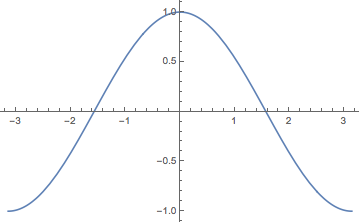
\includegraphics[scale=0.4]{cos_eo} & 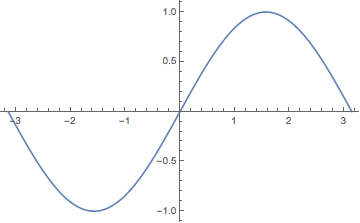
\includegraphics[scale=0.4]{sin_eo} & 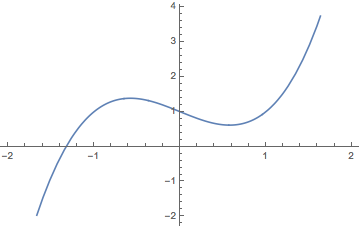
\includegraphics[scale=0.4]{cube_eo}\\
$f(x) = \cos{x}$ & $f(x) = \sin{x}$ & $f(x) = x^{3}-x +1$
\end{tabular}
\end{center}
\noindent\\
\indent We should recall that a function is \textit{even} when $f(x) = f(-x)$
for all $x$ in the domain of $f$. Graphically speaking, an \textit{even}
function is reflected across only the $y$-axis. By looking at the above graphs,
we can see that $f(x) = \cos{x}$ is an even function.\\
\indent A function is \textit{odd} when $-f(x) = f(-x)$ for all x in the domain
of $f$. Graphically speaking, the function is reflected across the $x$-axis and
the $y$-axis. From the above graphs, we can say that $f(x) = \sin{x}$ is an odd
function. Note that we can have a function that is neither odd nor even, but we
won't see much of this in the following problems. The reason that we want to
discuss odd and even functions here is because the integration that we will be
seeing later will be affected by the symmetry.\\\\
\indent The first type of series we will look at is the Full Fourier Series.
Note that this series is just a combination of a Fourier Sine Series and a
Fourier Cosine Series. A typical problem would look something like this:\\\\
\textbf{\textit{Ex:}} Find the corresponding Fourier Series for
\begin{gather*}
f(x)=
\begin{cases*}
L \qquad -L \leq x \leq 0\\
2x \qquad 0 \leq x \leq L
\end{cases*}
\end{gather*}
\indent \textbf{\textit{Solution:}} So we have a piecewise function here, but
that shouldn't throw us off too much; all we need to do is combine the integrals
for each part of the coefficient solution. Let's start by finding the terms for
the $cos$ series.
\begin{align*}
B_{0} &= \frac{1}{2L}\left[\int_{-L}^{0}Ldx + \int_{0}^{L}2xdx\right]\\
&= \frac{1}{2L}[2L^{2}]\\
&= L
\end{align*}
\noindent Now We need to find $B_{n}$, and then we will have our cosine part of
the series. The integration can get pretty messy, so we will skip some steps.
\begin{align*}
B_{n} &= \frac{1}{L}\left[\int_{-L}^{0}L\cos{\left(\frac{n\pi x}{L}\right)}dx + \int_{0}^{L}2x\cos{\left(\frac{n\pi x}{L}\right)}dx\right]\\
&= \frac{1}{L}\left[0 + \left(\frac{2L^{2}}{n^{2}\pi^{2}}\right)((-1)^{n} - 1)\right]\\
&= \frac{2L}{(n\pi)^{2}}((-1)^{n} - 1)
\end{align*}
\noindent Note that the sequence will be 0 for all $n = 2k$. This allows us to
substitute $2k+1$ for $n$, since we don't care about the $0$ terms. For our
cosine part of the series, we now have:
\begin{align*}
B_{n} &= \frac{2L}{(2k+1)^{2}\pi^{2}}((-1)^{2k+1}-1)\\
&= \frac{2L}{(2k+1)^{2}\pi^{2}}(-2)\\
&= \frac{-4L}{(2k+1)^{2}\pi^{2}}
\end{align*}
\noindent Now we need to find the sine part of the series. This is easier,
since we only need to find $A_{n}$.
\begin{align*}
A_{n} &= \frac{1}{L}\left[\int_{-L}^{0}L\sin{\left(\frac{n\pi x}{L}\right)}dx +
\int_{0}^{L}2x\sin{\left(\frac{n\pi x}{L}\right)}dx \right]\\
&= \frac{L}{n\pi}\left[-1-(-1)^{n}\right]
\end{align*}
\noindent Note that we can do a similar substitution here as we did with the
cosine series. This time, however, we will have $0$ for $n = 2k+1$ We now have:
\begin{align*}
A_{n} &= \frac{L}{2k\pi}\left[-1-(-1)^{2k}\right]\\
&= \frac{L}{2k\pi}\left[-1 - 1\right]\\
&= \frac{L}{2k\pi}\left[-2\right]\\
&= \frac{-2L}{2k\pi}
\end{align*}
\noindent Now we have all the parts that we need. Our final answer will be
the sum of all the parts:
\begin{align*}
f(x)&\sim \frac{L}{2} + \sum_{k = 0}^{\infty}\left[\frac{-4L}{(2k+1)^{2}\pi^{2}}
\cos{\left(\frac{(2k + 1)\pi x}{L}\right)} \right] + \sum_{k =
0}^{\infty}\left[\frac{-2L}{2k\pi}\sin{\left(\frac{2k\pi x}{L}\right)} \right]\\
&\sim \frac{L}{2} + \sum_{k = 0}^{\infty}\left[\frac{-4L}{(2k+1)^{2}\pi^{2}}
\cos{\left(\frac{(2k + 1)\pi x}{L}\right)} + \frac{-2L}{2k\pi}\sin{
\left(\frac{2k\pi x}{L}\right)} \right]
\end{align*}
\noindent And we are done.\\


\newpage
\indent Now lets take a look at a slightly more theoretical Fourier Series.\\
\noindent\textbf{\textit{Ex:}} Find the corresponding Fourier Series for\\
\[f(x)=\left|\cos{x}\right|\qquad -\pi\leq x \leq \pi\]
\indent\textbf{\textit{Solution:}} Before we dive into calculations here, let's
analyze the function at hand. We have the absolute value of $\cos{x}$. Usually,
$\cos$ would be an odd function, which would imply that our $\cos$ series
component to the whole Fourier Series would be $0$. However, the absolute value
makes our function even, and as such the $\sin$ component of the series will be
$0$. That's good news for us, because now we don't have to find $a_{n}$; we
actually only have a Fourier Cosine Series here. Recall that we have a formula
for $b_{n}$ and $b_{0}$, and that our general solution will have the form of
\[\frac{b_{0}}{2} + \sum_{n=1}^{\infty}[b_{n}\cos{\left(\frac{n\pi x}{L}\right)}]\]
\noindent Our function is bounded by $\pi$, so we really have $L= \pi$. This gives us:
\[\frac{b_{0}}{2} + \sum_{n=1}^{\infty}[b_{n}\cos{\left(nx\right)}]\]
\noindent Let's go ahead and find our $b_{0}$:
\begin{align*}
b_{0} &= \frac{1}{\pi}\int_{-\pi}^{\pi}\left|\cos{x}\right|dx\\
&= \frac{2}{\pi}\int_{0}^{\pi}\left|\cos{x}\right|dx\\
&= \frac{4}{\pi}\int_{0}^{\frac{\pi}{2}}\left|\cos{x}\right|dx\\
&= \frac{4}{\pi}\left[\sin{\frac{\pi}{2}} - \sin{0}\right]\\
&= \frac{4}{\pi}
\end{align*}
\noindent We know that since the function is even, we can say that the the
integral of the entire range is really twice the integral of half the range.
Since we are dealing with the cosine function, we actually have four times a
quarter of the range. If we take a look at a graph, this may make more sense:\\
\begin{center}
\begin{tabular}{c c}
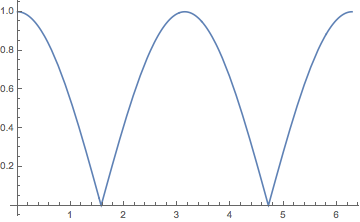
\includegraphics[scale=0.5]{cos_abs} & 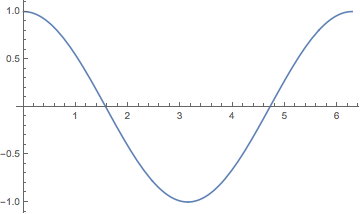
\includegraphics[scale=0.5]{cos}\\
$f(x) = |\cos{x}|$ on $[0,2\pi]$ & $f(x) = \cos{x}$ on $[0,2\pi]$
\end{tabular}
\end{center}
\noindent\\ You can see that the section of the graph from
$[\frac{\pi}{2},\frac{3 \pi}{2}]$ is positive for the $|\cos{x}|$, but negative
for $\cos{x}$. If we simply integrated the $|\cos{x}|$ over $[0,\pi]$, the
result would be 0, but graphically this result would not make any sense. Now
let's take a look at the $b_{n}$ term. Before we jump into the integration,
let's think about this function:
\[\left|\cos{x}\right| =
\begin{cases*}
\cos(x) \qquad 0\leq x \leq \frac{\pi}{2}\\
-\cos(x)\quad  \frac{\pi}{2}\ \leq x \leq \pi
\end{cases*}
\]
\noindent Now we can set up the formula for the $b_{n}$ term. We have as follows:
\begin{align*}
b_{n} &= \frac{2}{\pi}\left[ \int_{0}^{\frac{\pi}{2}} \cos{x}\cos{nx}dx - \int_{\frac{\pi}{2}}^{\pi}
\cos{x}\cos{nx}dx \right]\\
&= \frac{2}{\pi} \left[ \frac{-2 \cos{\left(\frac{n\pi}{2}\right)} + \sin{\left(n\pi\right)}}{n^{2} -
1}\right]\\
\end{align*}
\noindent Note that (as we have seen before) the sine term disappears; however,
the more interesting part is what happens with our cosine term. The value of
$\cos{\left(\frac{n\pi}{2}\right)}$ will be 0 at all odd $n$, or for all
$n = 2k + 1$. So, we will let our $n = 2k$. This gives us:
\begin{align*}
b_{n} &= \frac{2}{\pi} \left[ \frac{-2 \cos{\left(k \pi \right)}}{(2k)^{2} - 1}\right]\\
&= -\frac{4}{\pi}\left[\frac{(-1)^{k}}{(2k)^{2}-1}\right]
\end{align*}
\noindent And that leaves us with the final result
\[
f(x)\sim \frac{2}{\pi} - \sum_{k=0}^{\infty}\left[\frac{4}{\pi}\left[\frac{(-1)^{k}}{(2k)^{2}-1}\right]
\cos{\left(\frac{2k\pi}{2}\right)}\right]
\]
And we are done.
\newpage
\subsection{Convergence of Fourier Series}
\indent Up to this point, we have found a Fourier series and left our solutions
at that. We will now look into the convergence of a Fourier series. This topic
includes two questions:
\begin{enumerate}
\item Does the series converge?
\item If the series converges, to what value does it converge?
\end{enumerate}
\noindent Before we jump into convergence, we need to review some ideas.
\begin{enumerate}
\item \textit{\textbf{Jump Discontinuity:}} To say that $f(x)$ has a jump
discontinuity at $x = a$ is to say that
\[
\lim_{x \to a^{-}}f(x) \neq \lim_{x \to a^{+}}f(x)
\]
Where both the limit from the left and the limit from the right exist.
\item \textit{\textbf{Piecewise Smooth:}} A function $f(x)$ is said to be
piecewise smooth if the function can be broken into two distinct intervals, and
on each interval both $f(x)$ and $f^{'}(x)$ are continuous.
\item \textit{\textbf{Periodic Extension:}} The periodic extension of $f(x)$ on
$[-L,L]$ is the repetition of the function on intervals on periods to the left
and right of $[-L,L]$.
\end{enumerate}
\indent With these definitions, we can lay out a general rule for convergence of
a Fourier series. We won't give a proof of these rules for the time being. We
just need them to lay out some groundwork for the rest of the information we
will present on Fourier series. We have the following:
\begin{quote}
Suppose $f(x)$ is a function, and that $f(x)$ is piecewise smooth on the interval
$[-L,L]$. The corresponding Fourier series for $f(x)$ converges to either
\begin{enumerate}
\item the periodic extension of $f(x)$, if $f(x)$ is continuous, or
\item the average of the two one-sided limits, if the periodic extension of
$f(x)$ has a jump discontinuity at $x = a$.
\end{enumerate}
\end{quote}
\noindent We should note that the second condition can be expressed by the formula
\[\frac{1}{2}\left[\lim_{x \to a^{-}}f(x) + \lim_{x \to a^{+}}f(x)\right]\]
which gives us a nice way to calculate the value to which the series converges
if we happen to meet the criteria in (2). Let's take a look at some examples.\\\\


\noindent\textbf{\textit{Ex:}} Find the Fourier series for the following
equation, and determine if the series converges. If it does, tell where the
series will converge.
\[ f(x) =
\begin{cases}
L \qquad\qquad -L \leq x \leq 0\\
2x \qquad\qquad 0 \leq x \leq L
\end{cases}
\]
\indent\textbf{\textit{Solution:}} We will go ahead and skip the details of
finding the Fourier series for this function. If you do want to find it, you
will have to find a full piecewise Fourier series. For this particular $f(x)$,
we have:
\begin{align*}
f(x) &\sim L + \sum_{n=1}^{\infty}\left[\frac{2L}{n^{2}\pi^{2}}([-1]^{n}-1)\cos{\left(\frac{n\pi
x}{L}\right)}\right] - \sum_{n=1}^{\infty}\left[\frac{L}{n\pi}(1 + [-1]^{n})\sin{\left(\frac{n\pi
x}{L}\right)}\right]
\end{align*}
\noindent Notice that we didn't simplify this solution to a nicer form.
If we evaluate this series, we will run across terms where the series is 0, but
that is okay for now. This function is also defined as a piecewise function,
and on both intervals ($[-L,0]$ and $[0,L]$), $f(x)$ is continuous. In other
words, $f(x)$ is piecewise smooth, so we know that this series converges. Now
let's take a look at the graph of $f(x)$ on an arbitrary interval of $[-1,1]$.
\begin{center}
\begin{tabular}{c}
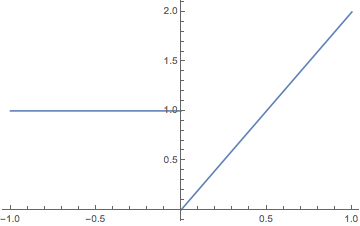
\includegraphics[scale=0.6]{pw_graph_01}\\
$
f(x) =
\begin{cases}
1 \qquad\qquad -1 \leq x \leq 0\\
2x \qquad\qquad 0 \leq x \leq 1
\end{cases}
$
\end{tabular}
\end{center}
\noindent We can see that there is a jump in the graph at $x = 0$. In other
words, there is a jump discontinuity at $x = 0$, and that means that we need to
use (2) in order to find the value of convergence. We will let $\sum$ stand in
for our entire series. We have:
\begin{align*}
\sum &\to \frac{1}{2}\left[\lim_{x\to 0}L + \lim_{x\to0}2x\right]\\
&\to \frac{1}{2}[L + 0]\\
&\to \frac{L}{2}
\end{align*}
\noindent So, at $x=0$, the series converges to $\frac{L}{2}$. We are not done
yet, however. Now, we need to consider the periodic extension of the series. The
function will repeat every $[-L,L]$, so we need to look at what the convergence
of the series looks like at $-L$ and $L$. Let's take a look:
\begin{alignat*}{3}
\sum&\to\frac{1}{2}\left[\lim_{x\to-L^{-}}f(x) + \lim_{x\to-L^{+}}f(x)\right] \qquad\qquad \sum&&\to
\frac{1}{2}\left[\lim_{x\to L^{-}}f(x) + \lim_{x\to L^{+}}f(x)\right]\\
&\to \frac{1}{2}[2L + L] &&\to \frac{1}{2}[2L + L]\\
&\to\frac{3L}{2} &&\to\frac{3L}{2}
\end{alignat*}
\noindent And we are done.
